% Created 2025-05-17 Sat 18:49
% Intended LaTeX compiler: pdflatex
\documentclass[11pt]{article}
\usepackage[utf8]{inputenc}
\usepackage[T1]{fontenc}
\usepackage{graphicx}
\usepackage{longtable}
\usepackage{wrapfig}
\usepackage{rotating}
\usepackage[normalem]{ulem}
\usepackage{amsmath}
\usepackage{amssymb}
\usepackage{capt-of}
\usepackage{hyperref}
\usepackage{mathptmx}  % Times font
\usepackage{helvet}   % Helvetica font
\renewcommand{\familydefault}{\sfdefault} % Sans-serif as default
\usepackage{titlesec}
\usepackage{lmodern}
\usepackage{amsmath}
\author{Serob Tigranyan}
\date{\today}
\title{Discrete Mathematics}
\hypersetup{
 pdfauthor={Serob Tigranyan},
 pdftitle={Discrete Mathematics},
 pdfkeywords={},
 pdfsubject={},
 pdfcreator={Emacs 29.4 (Org mode 9.7.11)}, 
 pdflang={English}}
\begin{document}

\maketitle
\tableofcontents

\newpage
\section{Task 1}
\label{sec:orgf3b1811}
We are given:
\[
A = \{ 1, 2, 3, 4, 5 \}
\]

And a relation matrix \(a\) where \(R \subseteq A \times A\):
\[
a =
 \begin{bmatrix}
 1 & 0 & 0 & 1 & 0 \\
 0 & 0 & 1 & 0 & 1 \\
 1 & 0 & 1 & 0 & 0 \\
 1 & 0 & 0 & 1 & 0 \\
 0 & 1 & 0 & 0 & 0
 \end{bmatrix}
\]

We need to find whether relation \(a\) is \textbf{reflextive}, \textbf{symmtetric} and \textbf{transitive}, if not then find their \textbf{closures} respectively.
\subsection{Reflexivity}
\label{sec:org9da59d8}
A relation is \textbf{reflexive} if every element is related to itself, e.g., \(a_{ii} = 1\) for all \(i\).

This means that the diagonal elements are all 1's, but it's not in our case therefore relation \(a\) is \textbf{not reflexive}.
\subsubsection{Reflexive Closure}
\label{sec:org2f1e6bd}
\textbf{Reflexive closure} for relation \(a\) would be \(a_{ref}\) where all the diagonal elements are 1's:

\[
a_{ref} =
 \begin{bmatrix}
 1 & 0 & 0 & 1 & 0 \\
 0 & 1 & 1 & 0 & 1 \\
 1 & 0 & 1 & 0 & 0 \\
 1 & 0 & 0 & 1 & 0 \\
 0 & 1 & 0 & 0 & 1
 \end{bmatrix}
\]
\subsection{Symmetry}
\label{sec:org07b5d17}
A relation is \textbf{symmetric} if \(a_{ij} = a_{ji}\). \\
We can check this by transposing our relation matrix and if \(T(a) = a\) then the relation is \textbf{symmetric}:
\[
T(a) =
 \begin{bmatrix}
 1 & 0 & 1 & 1 & 0 \\
 0 & 0 & 0 & 0 & 1 \\
 0 & 1 & 1 & 0 & 0 \\
 1 & 0 & 0 & 1 & 0 \\
 0 & 1 & 0 & 0 & 0
 \end{bmatrix}
\]

We can clearly observe that the transposed matrix differs from the original relation matrix therefore:
\[
T(a) \neq a
\]

So the relation \(a\) is \textbf{not symmetric}.
\subsubsection{Symmetric Closure}
\label{sec:org0f13d67}
The \textbf{symmetric closure} for relation \(a\) would be \(a_{sym}\) where every \(a_{ij} = a_{ji} = 1\):

\[
a_{sym} =
 \begin{bmatrix}
 1 & 0 & 0 & 1 & 0 \\
 0 & 1 & 1 & 0 & 1 \\
 1 & 0 & 1 & 0 & 0 \\
 1 & 0 & 0 & 1 & 0 \\
 0 & 1 & 0 & 0 & 1
 \end{bmatrix}
\]
\subsection{Transitivity}
\label{sec:orgf3264cc}
A relation is \textbf{transitive} if whenever \((i,j) \in R\) and \((j, k) \in R\), then \((i,k) \in R\). \\
We can easily check by taking the \textbf{boolean} square of the relation matrix \(a\):
\[
a^2 =
 \begin{bmatrix}
 1 & 0 & 0 & 1 & 0 \\
 1 & 1 & 1 & 0 & 0 \\
 1 & 0 & 1 & 1 & 0 \\
 1 & 0 & 0 & 1 & 0 \\
 0 & 0 & 1 & 0 & 1
 \end{bmatrix}
\]

If all the 1's in \(a^2\) exists in \(a\) then the relation is \textbf{transitive}, but this is not the case for us therefore the relation \(a\) is \textbf{not transitive}.
\subsubsection{Transitive Closure}
\label{sec:orge972809}
We can use Warshall's algorithm to find the transitive closure for relation \(a\).
After applying Warshall's algorithm to our initial relation matrix we get:
\[
a_{trans} =
\begin{bmatrix}
1 & 0 & 0 & 1 & 0 \\
1 & 1 & 1 & 1 & 1 \\
1 & 0 & 1 & 1 & 0 \\
1 & 0 & 0 & 1 & 0 \\
1 & 1 & 1 & 1 & 1
\end{bmatrix}
\]

\newpage
\section{Task 2}
\label{sec:org3dbf359}
We are asked to find how many integers below or equal to 1000 are divisible by 8, 22 or 32.

Let:
\begin{itemize}
\item \(A\): Numbers divisible by 8
\item \(B\): Numbers divisible by 22
\item \(C\): Numbers divisible by 32
\end{itemize}
\subsection{Calculate the numbers that 1000 is divisible by each number}
\label{sec:orgb0bfd42}
We start by finding how many nymbers up to 1000 are divisible by: \\

\(8\): Divide 1000 by 8:
  \[
   \left\lfloor \frac{1000}{8} \right\rfloor = 125
   \]

\(22\): Divide 1000 by 22:
  \[
   \left\lfloor \frac{1000}{22} \right\rfloor = 45
   \]

\(32\): Divide 1000 by 32:
  \[
   \left\lfloor \frac{1000}{22} \right\rfloor = 31
   \]
\subsection{Substract overlap}
\label{sec:orge2ba73e}
Then we will need to subtract the overlap numbers counted twice. \\
Some numbers are disible by both 8 and 22, or 8 and 32, etc. \\
We subtract them so we don't count them twice. \\

To do this, we find how many numbers are divisible by both pairs:
\begin{itemize}
\item 8 and 22:
Find LCM (Least Common Multiple) of 8 and 22
\[
  LCM(8, 22) = 88
  \]
\[
  \left\lfloor \frac{1000}{88} \right\rfloor = 11
  \]

\item 8 and 32:
Find LCM of 8 and 32
\[
  LCM(8, 32) = 32
  \]
\[
  \left\lfloor \frac{1000}{32} \right\rfloor = 31
  \]

\item 22 and 32:
Find LCM of 22 and 32
\[
  LCM(22, 32) = 352
  \]
\[
  \left\lfloor \frac{1000}{352} \right\rfloor = 2
  \]
\end{itemize}
\subsection{Add back numbers counted 3 times}
\label{sec:org4a38d6f}
Some numbers are divisible by all three so we add these back because we subtracted them earlier.
\begin{itemize}
\item \(LCM(8, 22, 32) = 352\)
\end{itemize}
\[
\left\lfloor \frac{1000}{352} \right\rfloor = 2
\]
\subsection{Putting it all together using Inclusion-Exclusion Formula}
\label{sec:orgeaef607}
The \textbf{Inclusion-Exclusion} Formula states the following:
\[
\left|A \cup B \cup C \right| = \left|A\right| + \left|B\right| + \left|C \right| - \left|A \cap B \right| - \left|A \cap C \right| - \left|B \cap C \right| + \left|A \cap B \cap C \right|
\]

Plug in our values:
\begin{itemize}
\item \(A = 125\)
\item \(B = 45\)
\item \(C = 31\)
\item \(AB = 11\)
\item \(AC = 31\)
\item \(BC = 2\)
\item \(ABC = 2\)
\end{itemize}

Therefore:
\[
125 + 45 + 31 - 11 - 31 - 2 + 2 = 159
\]

\newpage
\section{Task 3}
\label{sec:org8376763}
We are given graphs \(H\) and \(G\):
\begin{center}
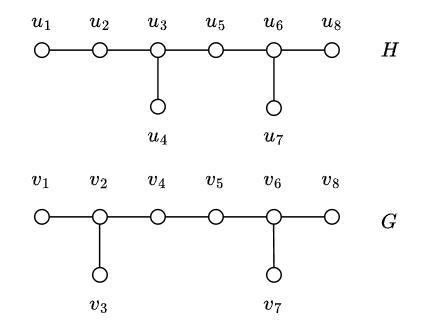
\includegraphics[width=0.6\textwidth]{./grappherr.png}
\end{center}

We must determine if the given graphs are \textbf{isomorphic}.
First we recall the definition of two isomorphic graphs: \\

Let \(G_1 = (V_1,E_1)\) \& \(G_2 = (V_2, E_2)\) be two simple graphs where:
\begin{itemize}
\item \(V_1, V_2\) are the sets of vertices
\item \(E_1, E_2\) are the sets of edges
\end{itemize}

Then \(G_1\) \& \(G_2\) are \textbf{isomorphic} if there exists a bijective function \(\varphi : V_1 \rightarrow V_2\) such that:
\begin{center}
\begin{tabular}{l}
\(\{u, v\} \in E_1\), if any only if \(\{\varphi\left(u\right), \varphi\left(v\right)\} \in E_2\)\\
\end{tabular}
\end{center}

In simpiler terms \(G\) \& \(H\) are \textbf{isomorphic} if there exists a bijection function \(\varphi\) that directly maps \(G\)'s vertices to \(H\)'s vertices (and vice-versa) and that each degree of both vertices match. \\

In our case it is visually apparent that these two graphs are not \textbf{isomorphic}.
More specificaally, the degrees of \(u_3, v_3\) do not match, \(u_3\) has degree of two while \(v_3\) has degree of just one. \\
Therefore these two graphis are not \textbf{isomorphic}.
\end{document}
